\section{Zbiory symplicjalne i nerw kategorii}\label{cat:sec:simplicial-sets}

Zbiory symplicjalne opisują obiekty za pomocą sympleksów wszystkich wymiarów, ich ścian i degeneracji. W odróżnieniu od abstrakcyjnego kompleksu symplicjalnego dopuszczają różne sympleksy o tych samych wierzchołkach. Są presnopami na pewnej szczególnej małej kategorii (por. definicja~\ref{cat:def:presheaf}). Konstrukcja nerwu pozwala zakodować w takim presnopie obiekty, morfizmy i składanie kategorii zwykłej.

\subsection{Kategoria sympleksów}

\begin{definicja}[Kategoria sympleksów]\label{cat:def:simplex-category}
Kategorię $\Delta$ tworzą niepuste skończone zbiory liniowo uporządkowane
\[
 [n]=\{0,1,\ldots,n\},\qquad n\geq 0,
\]
oraz wszystkie odwzorowania niemalejące między nimi. Składanie i identyczności są zwykłymi złożeniami i identycznościami funkcji. Zbiór $[n]$ traktujemy również jako kategorię, w której istnieje dokładnie jeden morfizm $i\to j$ dla $i\leq j$ i nie ma go dla $i>j$.
\end{definicja}
Funktory pomiędzy takimi kategoriami są dokładnie odwzorowaniami niemalejącymi: konieczność wynika z istnienia obrazu morfizmu $i\to j$, wystarczalność z jednoznaczności morfizmów o zadanych końcach.

\begin{definicja}[Koface i kodegeneracje]\label{cat:def:delta-generators}
Dla $n\geq1$ i $0\leq i\leq n$ niech $\delta^i:[n-1]\to[n]$ będzie rosnącą injekcją pomijającą $i$:
\[
 \delta^i(t)=
 \begin{cases}t&t<i,\\t+1&t\geq i.\end{cases}
\]
Dla $n\geq0$ i $0\leq i\leq n$ niech $\sigma^i:[n+1]\to[n]$ będzie surjekcją sklejącą $i$ oraz $i+1$:
\[
 \sigma^i(t)=
 \begin{cases}t&t\leq i,\\t-1&t>i.\end{cases}
\]
Wymiar dziedziny i przeciwdziedziny jest każdorazowo wyznaczony przez kontekst.
\end{definicja}

\begin{center}
\begin{tikzpicture}[>=stealth]
 \foreach \i in {0,1,2} {
  \node (a\i) at (1.35*\i,2.4) {$\i$};
  \node (b\i) at (1.35*\i,0) {$\i$};
 }
 \node (b3) at (4.05,0) {$3$};
 \draw[->] (a0)--(b0);
 \draw[->] (a1)--(b2);
 \draw[->] (a2)--(b3);
 \node at (2,-.8) {$\delta^1:[2]\to[3]$};
 \begin{scope}[xshift=6cm]
 \foreach \i in {0,1,2,3} \node (c\i) at (1.35*\i,2.4) {$\i$};
 \foreach \i in {0,1,2} \node (d\i) at (1.35*\i,0) {$\i$};
 \draw[->] (c0)--(d0);
 \draw[->] (c1)--(d1);
 \draw[->] (c2)--(d1);
 \draw[->] (c3)--(d2);
 \node at (2,-.8) {$\sigma^1:[3]\to[2]$};
 \end{scope}
\end{tikzpicture}
\end{center}

\begin{twierdzenie}[Rozkład morfizmu w $\Delta$]\label{cat:thm:delta-factorization}
Każde odwzorowanie niemalejące $\theta:[m]\to[n]$ ma jedyny rozkład $\theta=\iota\pi$, gdzie $\pi:[m]\to[r]$ jest surjekcją niemalejącą, a $\iota:[r]\to[n]$ rosnącą injekcją. Każda taka injekcja jest złożeniem kofac, a każda taka surjekcja złożeniem kodegeneracji (dopuszczamy puste złożenie).
\end{twierdzenie}
\begin{proof}
Niech obraz $\theta$ składa się z elementów $y_0<\cdots<y_r$. Jest niepusty, gdyż $[m]$ jest niepusty. Definiujemy $\iota(j)=y_j$ i $\pi(t)=j$ wtedy i tylko wtedy, gdy $\theta(t)=y_j$. Surjektywność $\pi$ wynika z definicji obrazu, a monotoniczność z monotoniczności $\theta$ i ścisłej monotoniczności $\iota$. Mamy $\theta(t)=\iota(\pi(t))$. W każdym rozkładzie tego rodzaju obraz injekcji jest obrazem $\theta$, ponieważ pierwszy czynnik jest surjekcją. Rosnąca enumeracja obrazu jest jedyna, zatem jedyne są $r$ i $\iota$. Injektywność $\iota$ wymusza jednoznaczność $\pi$.

Jeśli $\iota:[r]\to[n]$ nie jest surjekcją, wybieramy pominięty element $i$. Obraz $\delta^i:[n-1]\to[n]$ zawiera obraz $\iota$, więc istnieje jedyna rosnąca injekcja $\iota':[r]\to[n-1]$ z $\delta^i\iota'=\iota$: przypisujemy każdemu elementowi jego jedyny przeciwobraz przez $\delta^i$. Indukujemy względem $n-r$, przy czym dla $n=r$ rosnąca bijekcja jest identycznością.

Jeśli surjekcja $\pi:[m]\to[r]$ nie jest injekcją, istnieje $i<m$ z $\pi(i)=\pi(i+1)$: każde włókno odwzorowania niemalejącego jest przedziałem w porządku, więc włókno zawierające co najmniej dwa elementy zawiera dwa kolejne. Funkcja $\pi$ jest stała na włóknach $\sigma^i:[m]\to[m-1]$. Definiujemy $\pi'(j)=\pi(t)$ dla dowolnego $t$ spełniającego $\sigma^i(t)=j$; niezależność wyboru wynika ze stałości na włóknach. Funkcja $\pi'$ jest surjekcją i jest niemalejąca, ponieważ włókna $\sigma^i$ są uporządkowane zgodnie z ich wartościami. Mamy $\pi=\pi'\sigma^i$. Indukujemy względem $m-r$, z identycznością jako przypadkiem $m=r$.
\end{proof}

\subsection{Zbiory symplicjalne}

\begin{definicja}[Zbiór symplicjalny]\label{cat:def:simplicial-set}
Zbiór symplicjalny jest funktorem $X:\Delta^{\mathrm{op}}\to\Set$. Zapisujemy $X_n=X([n])$. Dla $\theta:[m]\to[n]$ piszemy $\theta^*=X(\theta):X_n\to X_m$; w tym zapisie argument $X$ jest morfizmem w kategorii przeciwnej odpowiadającym $\theta$. Elementy $X_n$ nazywamy $n$-sympleksami. Operatory ścian i degeneracji to odpowiednio
\[
 d_i=(\delta^i)^*:X_n\to X_{n-1},\qquad
 s_i=(\sigma^i)^*:X_n\to X_{n+1}.
\]
Morfizmem zbiorów symplicjalnych jest transformacja naturalna. Otrzymujemy kategorię $\mathbf{sSet}=[\Delta^{\mathrm{op}},\Set]$.
\end{definicja}

Z kontrawariancji wynika $(\theta\psi)^*=\psi^*\theta^*$. W szczególności nie wolno zamieniać kolejności operatorów przy odczytywaniu relacji w $\Delta$.

\begin{stwierdzenie}[Tożsamości symplicjalne]\label{cat:prop:simplicial-identities}
Dla wszystkich dopuszczalnych indeksów i wymiarów zachodzą
\begin{equation}\label{cat:eq:simplicial-identities}
\begin{aligned}
 d_i d_j&=d_{j-1}d_i &&(i<j),\\
 s_i s_j&=s_{j+1}s_i &&(i\leq j),\\
 d_i s_j&=
 \begin{cases}
 s_{j-1}d_i&i<j,\\
 \id&i=j\ \text{lub}\ i=j+1,\\
 s_j d_{i-1}&i>j+1.
 \end{cases}
\end{aligned}
\end{equation}
\end{stwierdzenie}
\begin{proof}
Pierwsza relacja wynika z $\delta^j\delta^i=\delta^i\delta^{j-1}$ dla $i<j$: obie strony są rosnącymi injekcjami o obrazie pomijającym dokładnie $i,j$ w końcowym zbiorze. Na lewej stronie druga injekcja pomija $j$ i wysyła $i$ na $i$, na prawej pomija $i$ i wysyła $j-1$ na $j$. Rosnąca enumeracja tego samego obrazu jest jedyna.

Dla drugiej relacji porównujemy $\sigma^j\sigma^i$ oraz $\sigma^i\sigma^{j+1}$, dla $i\leq j$. Surjekcja niemalejąca jest wyznaczona przez indeksy $t$, dla których jej wartości w $t,t+1$ są równe: zaczyna się od zera, a na pozostałych indeksach zwiększa wartość o jeden, gdyż jest surjekcją. Dla $i<j$ pierwsze złożenie ma takie indeksy $i,j+1$, ponieważ $\sigma^i$ skleja $i,i+1$, a para sklejona przez $\sigma^j$ odpowiada pierwotnej parze $j+1,j+2$. Drugie złożenie skleja tę samą parę $j+1,j+2$ oraz $i,i+1$. Dla $i=j$ obie strony sklejają trójkę $i,i+1,i+2$, więc mają te same indeksy $i,i+1$. Otrzymujemy równość.

W relacji mieszanej rozważamy $\sigma^j\delta^i$. Gdy $i=j$ lub $i=j+1$, injekcja usuwa jeden z dwóch elementów sklejanych przez $\sigma^j$, więc złożenie jest niemalejącą bijekcją tego samego zbioru, czyli identycznością. Dla pozostałych przypadków złożenie pomija wartość $\sigma^j(i)$ i skleja jedną parę kolejnych elementów dziedziny. Dla $i<j$ pominięta wartość to $i$, a sklejane indeksy to $j-1,j$; takie same dane ma $\delta^i\sigma^{j-1}$. Dla $i>j+1$ pominięta wartość to $i-1$, a sklejane indeksy to $j,j+1$; takie same dane ma $\delta^{i-1}\sigma^j$. W obu przypadkach obraz i sklejane indeksy jednoznacznie wyznaczają odwzorowanie, przez rozkład z twierdzenia~\ref{cat:thm:delta-factorization}. Stosując kontrawariantny funktor $X$ do wszystkich uzyskanych równości, odwracamy kolejność składania i dostajemy~\eqref{cat:eq:simplicial-identities}.
\end{proof}

\begin{definicja}[Sympleks zdegenerowany]\label{cat:def:degenerate-simplex}
Sympleks $x\in X_n$ jest zdegenerowany, jeśli dla pewnego $i$ i $y\in X_{n-1}$ mamy $x=s_i y$. W przeciwnym razie jest niezdegenerowany. Wszystkie $0$-sympleksy są niezdegenerowane.
\end{definicja}
Z tożsamości $d_i s_i=\id=d_{i+1}s_i$ wynika injektywność $s_i$ oraz surjektywność tych dwóch operatorów ścian. Nie wynika stąd, że wszystkie ściany sympleksu niezdegenerowanego są niezdegenerowane.

\subsection{Sympleksy standardowe}

\begin{definicja}[Standardowy zbiór symplicjalny]\label{cat:def:standard-simplicial-simplex}
Dla $n\geq0$ definiujemy presnop reprezentowalny
\[
 \Delta[n]_m=\Hom_\Delta([m],[n]),\qquad
 \theta^*(u)=u\theta.
\]
Morfizm $\Delta[n]\to\Delta[k]$ indukowany przez $\varphi:[n]\to[k]$ działa przez składanie z $\varphi$ z lewej strony.
\end{definicja}

\begin{stwierdzenie}[Symplicjalna postać lematu Yonedy]\label{cat:prop:simplicial-yoneda}
Dla dowolnego zbioru symplicjalnego $X$ istnieje naturalna bijekcja
\[
 \Hom_{\mathbf{sSet}}(\Delta[n],X)\longrightarrow X_n,
 \qquad t\longmapsto t_n(\id_{[n]}).
\]
Sympleksy niezdegenerowane w $\Delta[n]_m$ to dokładnie rosnące injekcje $[m]\to[n]$.
\end{stwierdzenie}
\begin{proof}
Pierwsza teza jest szczególnym przypadkiem lematu Yonedy~\ref{cat:thm:yoneda-contra}. Jawnie, do $x\in X_n$ przypisujemy transformację o składowych $u\mapsto u^*x$. Naturalność wynika z $(u\theta)^*x=\theta^*u^*x$. Dla transformacji $t$ jej naturalność względem $u:[m]\to[n]$ daje $t_m(u)=u^*(t_n(\id_{[n]}))$, więc podane przyporządkowania są odwrotne. Naturalność względem $X$ i $[n]$ wynika z naturalności $t$ oraz ze wzoru na odwrotność.

Jeżeli $u:[m]\to[n]$ nie jest injekcją, to w rozkładzie z twierdzenia~\ref{cat:thm:delta-factorization} czynnik surjektywny nie jest identycznością. W jego rozkładzie można wyodrębnić pierwszą stosowaną kodegenerację, otrzymując $u=v\sigma^i$. Zatem $u=s_i v$ jest zdegenerowany. Odwrotnie, każde $s_i v=v\sigma^i$ przyjmuje tę samą wartość na $i,i+1$, więc nie jest injekcją.
\end{proof}

\begin{center}
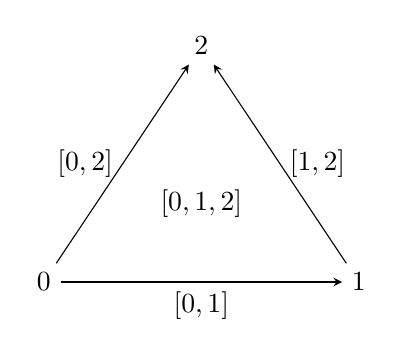
\begin{tikzpicture}[>=stealth]
 \node (a) at (0,0) {$0$};
 \node (b) at (4,0) {$1$};
 \node (c) at (2,3) {$2$};
 \draw[->] (a)--node[below] {$[0,1]$}(b);
 \draw[->] (b)--node[right] {$[1,2]$}(c);
 \draw[->] (a)--node[left] {$[0,2]$}(c);
 \node at (2,1) {$[0,1,2]$};
\end{tikzpicture}
\end{center}
Rysunek przedstawia niezdegenerowane sympleksy $\Delta[2]$: trzy wierzchołki, trzy krawędzie i jeden $2$-sympleks. Pozostałe sympleksy są degeneracjami tych sympleksów.

\subsection{Nerw kategorii}

\begin{definicja}[Nerw]\label{cat:def:category-nerve}
Dla małej kategorii $\mathcal C$ jej nerw to zbiór symplicjalny
\[
 N(\mathcal C)_n=\operatorname{Fun}([n],\mathcal C),
 \qquad \theta^*(F)=F\circ\theta.
\]
Złożenie z funktorem $H:\mathcal C\to\mathcal D$ daje morfizm symplicjalny $N(H):N(\mathcal C)\to N(\mathcal D)$.
\end{definicja}

\begin{stwierdzenie}[Opis sympleksów nerwu]\label{cat:prop:nerve-strings}
$n$-sympleks nerwu odpowiada jednoznacznie ciągowi $n$ składanych morfizmów
\[
 A_0\xrightarrow{f_1}A_1\xrightarrow{f_2}\cdots
 \xrightarrow{f_n}A_n.
\]
Dla $n\geq1$ operator $d_0$ usuwa pierwszy obiekt i pierwszy morfizm, a $d_n$ ostatni obiekt i ostatni morfizm. Dla $0<i<n$ operator $d_i$ usuwa obiekt $A_i$ i zastępuje dwa sąsiednie morfizmy przez $f_{i+1}f_i$. Operator $s_i$ powtarza $A_i$, wstawiając pomiędzy kopie morfizm $\id_{A_i}$.
\end{stwierdzenie}
\begin{proof}
Dla funktora $F:[n]\to\mathcal C$ bierzemy $A_i=F(i)$ i $f_i=F(i-1\to i)$. Każdy morfizm $i\to j$ dla $i<j$ jest złożeniem kolejnych strzałek w $[n]$, więc musi mieć obraz $f_j\cdots f_{i+1}$. Odwrotnie, ta formuła wraz z $F(i\to i)=\id_{A_i}$ określa funktor, ponieważ dla $i\leq j\leq k$ łączność i jednostkowość składania w $\mathcal C$ dają $F(j\to k)F(i\to j)=F(i\to k)$. Dla $n=0$ ciąg oznacza pojedynczy obiekt.

Prekompozycja z $\delta^i$ usuwa $i$ z ciągu obiektów. Gdy $0<i<n$, strzałka przekraczająca pominięty indeks ma obraz $F(i-1\to i+1)=f_{i+1}f_i$; w pozostałych miejscach obrazy strzałek się nie zmieniają. Dla skrajnych indeksów nie ma strzałki przekraczającej pominięty obiekt. Prekompozycja z $\sigma^i$ powtarza obiekt, a strzałkę $i\to i+1$ wysyła na identyczność w $i$, więc wstawia $\id_{A_i}$. Pozostałe strzałki są odpowiednimi strzałkami pierwotnego ciągu.
\end{proof}

\begin{center}
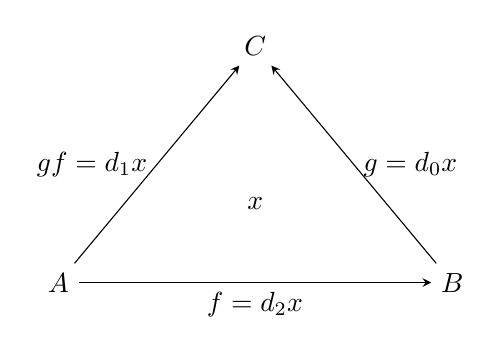
\begin{tikzpicture}[>=stealth]
 \node (a) at (0,0) {$A$};
 \node (b) at (5,0) {$B$};
 \node (c) at (2.5,3) {$C$};
 \draw[->] (a)--node[below] {$f=d_2x$}(b);
 \draw[->] (b)--node[right] {$g=d_0x$}(c);
 \draw[->] (a)--node[left] {$gf=d_1x$}(c);
 \node at (2.5,1) {$x$};
\end{tikzpicture}
\end{center}
W nerwie $2$-sympleks jest trójkątem przemiennym, a jego środkowa ściana koduje składanie.

\begin{twierdzenie}[Pełność i wierność nerwu]\label{cat:thm:nerve-fully-faithful}
Funktor $N:\mathbf{Cat}\to\mathbf{sSet}$ z kategorii małych kategorii jest pełny i wierny.
\end{twierdzenie}
\begin{proof}
Postkompozycja z funktorem $H$ komutuje z prekompozycją z dowolnym $\theta$ z $\Delta$, więc $N(H)$ jest transformacją naturalną; zachowywanie identyczności i składania wynika ze składania funktorów. Niech $t:N(\mathcal C)\to N(\mathcal D)$ będzie morfizmem symplicjalnym. Definiujemy $H$ na obiektach przez $t_0$ i na morfizmach przez $t_1$. Dla $f:A\to B$ mamy $d_1f=A$ i $d_0f=B$. Komutowanie $t$ z tymi ścianami pokazuje, że $Hf:HA\to HB$. Ponieważ $s_0A=\id_A$, komutowanie z $s_0$ daje $H(\id_A)=\id_{HA}$.

Dla $f:A\to B$, $g:B\to C$ niech $x\in N(\mathcal C)_2$ będzie ciągiem $(f,g)$. Ściany $d_2t_2(x)$ i $d_0t_2(x)$ to odpowiednio $Hf,Hg$. Na mocy stwierdzenia~\ref{cat:prop:nerve-strings} sympleks $t_2(x)$ jest więc ciągiem $(Hf,Hg)$. Jego środkowa ściana daje
\[
 H(gf)=t_1(d_1x)=d_1t_2(x)=Hg\,Hf.
\]
Otrzymujemy funktor $H$. Dla dowolnego $n$-sympleksu $x$ jego kolejne krawędzie otrzymujemy przez prekompozycję z injekcjami $[1]\to[n]$ wysyłającymi $0,1$ na $i-1,i$. Naturalność $t$ względem tych injekcji oznacza, że kolejnymi krawędziami $t_n(x)$ są obrazy przez $H$ kolejnych krawędzi $x$. Dla $n\geq1$ ciąg tych krawędzi wyznacza sympleks jednoznacznie; dla $n=0$ równość wynika z definicji $H$. Zatem $t=N(H)$. Jednoznaczność $H$ wynika z jego składowych na obiektach i morfizmach, wymuszonych przez $t_0,t_1$.
\end{proof}

\begin{przyklad}[Nerw porządku i nerw grupy]\label{cat:ex:nerve-poset-group}
Dla zbioru częściowo uporządkowanego $P$ traktowanego jako kategoria $N(P)_n$ jest zbiorem niemalejących ciągów $p_0\leq\cdots\leq p_n$. Degeneracja powtarza element; ciąg jest niezdegenerowany dokładnie wtedy, gdy wszystkie kolejne nierówności są ostre.

Dla grupy $G$ traktowanej jako kategoria o jednym obiekcie, z morfizmami $G$ i składaniem zgodnym z mnożeniem, $N(G)_n=G^n$ (dla $n=0$ singleton). Ściany skrajne usuwają skrajny czynnik, ściana wewnętrzna mnoży $g_{i+1}g_i$, a degeneracja wstawia jednostkę grupy. Jeśli $G$ jest nietrywialna, nerw ma wiele krawędzi o tych samych końcach, co pokazuje różnicę między zbiorami symplicjalnymi i abstrakcyjnymi kompleksami symplicjalnymi. Oba opisy wynikają ze stwierdzenia~\ref{cat:prop:nerve-strings}.
\end{przyklad}


\subsection{Jednoznaczność rozkładu sympleksu na degenerację}

\begin{lemat}[Lemat Eilenberga--Zilbera]\label{cat:lem:ez-degeneracy}
Dla każdego zbioru symplicjalnego $X$ i każdego $x\in X_n$ istnieje dokładnie jedna para $(\pi,y)$, gdzie $\pi:[n]\to[r]$ jest surjekcją w $\Delta$, a $y\in X_r$ jest sympleksem niezdegenerowanym, taka że $x=\pi^*y$.
\end{lemat}
\begin{proof}
Istnienie dowodzimy indukcyjnie względem $n$. Jeżeli $x$ jest niezdegenerowany, bierzemy $r=n$, $\pi=\id_{[n]}$, $y=x$. W przeciwnym razie $x=s_i z=(\sigma^i)^*z$ dla pewnego $z\in X_{n-1}$. Z założenia indukcyjnego $z=\rho^*y$ dla surjekcji $\rho:[n-1]\to[r]$ i niezdegenerowanego $y$. Wówczas $x=(\rho\sigma^i)^*y$, a $\rho\sigma^i$ jest surjekcją. Przypadek $n=0$ należy do pierwszego przypadku.

Dla jednoznaczności załóżmy, że
\[
 x=\pi^*y=\tau^*z,\qquad
 \pi:[n]\twoheadrightarrow[r],\quad
 \tau:[n]\twoheadrightarrow[q],
\]
gdzie $y,z$ są niezdegenerowane. Każda surjekcja niemalejąca ma rosnącą sekcję: z każdego niepustego włókna wybieramy jeden element, a włókna są uporządkowane w kolejności odpowiadającej ich wartościom. Dla dowolnej takiej sekcji $a:[r]\to[n]$ surjekcji $\pi$ zachodzi
\[
 y=a^*\pi^*y=a^*\tau^*z=(\tau a)^*z.
\]
Morfizm $\tau a$ musi być injekcją. W przeciwnym razie jego rozkład na surjekcję i injekcję z twierdzenia~\ref{cat:thm:delta-factorization} miałby nieidentycznościowy czynnik surjektywny. Zapisując ten czynnik jako złożenie kodegeneracji i wyodrębniając pierwszą stosowaną kodegenerację, otrzymalibyśmy $y=s_i w$ dla pewnego $w$, wbrew niezdegenerowaniu $y$.

Przypuśćmy, że $\pi(i)<\pi(i+1)$, lecz $\tau(i)=\tau(i+1)$ dla pewnego $0\leq i<n$. Wybieramy sekcję $a$ surjekcji $\pi$, która zawiera w obrazie zarówno $i$, jak i $i+1$: należą one do różnych włókien, z pozostałych włókien wybieramy dowolne elementy. Wówczas $\tau a$ nie jest injekcją, sprzecznie z poprzednim akapitem. Wykazaliśmy implikację
\[
 \tau(i)=\tau(i+1)\ \Longrightarrow\
 \pi(i)=\pi(i+1).
\]
Zamieniając role $(\pi,y)$ i $(\tau,z)$, otrzymujemy implikację odwrotną. Surjekcja niemalejąca zaczyna się od zera, a między kolejnymi argumentami zwiększa wartość o zero lub jeden. Jest więc wyznaczona przez zbiór indeksów, na których nie zwiększa wartości. Stąd $r=q$ oraz $\pi=\tau$. Dla dowolnej sekcji $a$ tej surjekcji mamy wreszcie $y=a^*x=z$.
\end{proof}

\begin{wniosek}\label{cat:cor:ez-degeneracy-decomposition}
Oznaczmy przez $X_r^{\mathrm{nd}}$ zbiór niezdegenerowanych $r$-sympleksów. Dla każdego $n$ istnieje bijekcja
\[
 \coprod_{r=0}^n\ \coprod_{\pi:[n]\twoheadrightarrow[r]}
 X_r^{\mathrm{nd}}\longrightarrow X_n,\qquad
 (\pi,y)\longmapsto\pi^*y,
\]
gdzie suma rozłączna przebiega po surjekcjach w $\Delta$.
\end{wniosek}
\begin{proof}
Surjektywność i injektywność tej funkcji są odpowiednio istnieniem i jednoznacznością w lemacie~\ref{cat:lem:ez-degeneracy}. Nie twierdzimy, że rozkład jest naturalny względem dowolnych morfizmów zbiorów symplicjalnych: obraz niezdegenerowanego sympleksu może być zdegenerowany.
\end{proof}

\subsection{Brzegi i rogi sympleksów}

\begin{definicja}[Brzeg i róg]\label{cat:def:simplicial-boundary-horn}
Brzeg $\partial\Delta[n]$ jest podzbiorem symplicjalnym $\Delta[n]$, którego $m$-sympleksy to odwzorowania $u:[m]\to[n]$ niebędące surjekcjami. Dla $n=0$ otrzymujemy pusty zbiór symplicjalny.

Dla $n\geq1$ i $0\leq k\leq n$ róg $\Lambda^k[n]$ jest podzbiorem symplicjalnym $\Delta[n]$ określonym przez
\[
 \Lambda^k[n]_m=
 \{u:[m]\to[n]\text{ w }\Delta:
       \text{ istnieje }i\ne k\text{ takie, że }i\notin\operatorname{im}u\}.
\]
Nazywamy go rogiem wewnętrznym, gdy $0<k<n$, i zewnętrznym, gdy $k=0$ lub $k=n$.
\end{definicja}
Oba warunki są zachowywane przez prekompozycję z dowolnym morfizmem $\theta$ kategorii $\Delta$, ponieważ $\operatorname{im}(u\theta)\subseteq\operatorname{im}u$. Definiują więc podfunktory presnopa $\Delta[n]$.

Kofaca $\delta^i$ indukuje morfizm $\Delta[n-1]\to\Delta[n]$, który w stopniu $m$ jest injekcją $v\mapsto\delta^iv$; jego obraz składa się dokładnie z odwzorowań pomijających $i$. Brzeg jest sumą wszystkich tych ścian, a róg $\Lambda^k[n]$ sumą ścian o indeksach $i\ne k$. Sumy podzbiorów są brane w każdym stopniu.

\begin{center}
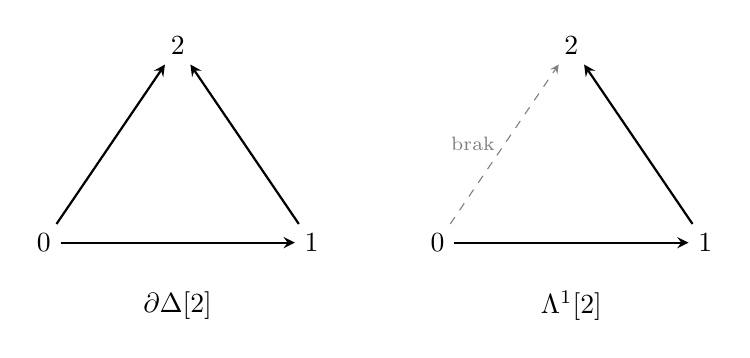
\begin{tikzpicture}[>=stealth]
 \begin{scope}
 \node (a) at (0,0) {$0$};
 \node (b) at (3.4,0) {$1$};
 \node (c) at (1.7,2.5) {$2$};
 \draw[->,thick] (a)--(b);
 \draw[->,thick] (b)--(c);
 \draw[->,thick] (a)--(c);
 \node at (1.7,-.8) {$\partial\Delta[2]$};
 \end{scope}
 \begin{scope}[xshift=5cm]
 \node (a) at (0,0) {$0$};
 \node (b) at (3.4,0) {$1$};
 \node (c) at (1.7,2.5) {$2$};
 \draw[->,thick] (a)--(b);
 \draw[->,thick] (b)--(c);
 \draw[->,dashed,gray] (a)--node[left] {\scriptsize brak} (c);
 \node at (1.7,-.8) {$\Lambda^1[2]$};
 \end{scope}
\end{tikzpicture}
\end{center}
Róg wewnętrzny $\Lambda^1[2]$ zawiera krawędzie $0\to1$, $1\to2$ i ich wierzchołki. Krawędź $0\to2$ oraz $2$-sympleks nie należą do rogu. Linie przerywane oznaczają brakujące krawędzie, a nie dodatkowe morfizmy.

\begin{stwierdzenie}[Rodziny zgodnych ścian]\label{cat:prop:simplicial-compatible-faces}
Niech $n\geq1$ i $I\subseteq\{0,\ldots,n\}$. Oznaczmy przez $K_I$ sumę obrazów kofac o indeksach $i\in I$ w $\Delta[n]$. Morfizmy $K_I\to X$ odpowiadają bijektywnie rodzinom $(x_i)_{i\in I}$, $x_i\in X_{n-1}$, spełniającym dla $n\geq2$
\begin{equation}\label{cat:eq:compatible-faces}
 d_i x_j=d_{j-1}x_i\qquad(i<j,\ i,j\in I).
\end{equation}
Dla $n=1$ nie ma dodatkowego warunku zgodności.
\end{stwierdzenie}
\begin{proof}
Morfizm na każdej ścianie wyznacza sympleks $x_i$ przez lemat Yonedy (stwierdzenie~\ref{cat:prop:simplicial-yoneda}). Dla $i<j$ przecięcie ścian o indeksach $i,j$ składa się w stopniu $m$ z odwzorowań $[m]\to[n]$ pomijających oba indeksy. Dla $n\geq2$ jest to obraz jednej injekcji $\Delta[n-2]\to\Delta[n]$ odpowiadającej rosnącej enumeracji pozostałych wierzchołków. Enumerację tę można zapisać jako $\delta^j\delta^i=\delta^i\delta^{j-1}$. Ograniczenia morfizmów na obu ścianach odpowiadają więc $d_i x_j$ i $d_{j-1}x_i$. Dla $n=1$ przecięcie dwóch różnych ścian jest puste w każdym stopniu, ponieważ nie istnieje funkcja z niepustego $[m]$ do pustego zbioru.

Odwrotnie, z rodziny zgodnej budujemy morfizm w stopniu $m$: dla $u\in (K_I)_m$ wybieramy $i\in I$ pomijany przez $u$, zapisujemy jednoznacznie $u=\delta^i v$ i przypisujemy $v^*x_i$. Jeżeli $u$ pomija również $j$, warunek zgodności oznacza równość ograniczeń obu morfizmów na przecięciu, a więc wynik nie zależy od wyboru. Dla $\theta:[l]\to[m]$ ten sam indeks $i$ jest pomijany przez $u\theta$, a jego rozkład to $\delta^i(v\theta)$. Z kontrawariancji $(v\theta)^*x_i=\theta^*v^*x_i$, co daje naturalność. Każdy morfizm o zadanych ograniczeniach musi mieć taki wzór, zatem jest jedyny. Gdy $I=\varnothing$, istnieje dokładnie jeden morfizm z pustego zbioru symplicjalnego i dokładnie jedna pusta rodzina.
\end{proof}

\begin{definicja}[Wypełnienie rogu]\label{cat:def:horn-filler}
Wypełnieniem morfizmu $h:\Lambda^k[n]\to X$ nazywamy morfizm $\widetilde h:\Delta[n]\to X$, którego ograniczenie do $\Lambda^k[n]$ jest równe $h$. Analogicznie definiujemy wypełnienia brzegu.
\end{definicja}
W języku poprzedniego stwierdzenia wypełnienie rogu odpowiada sympleksowi $x\in X_n$ spełniającemu $d_i x=x_i$ dla wszystkich $i\ne k$. Nie żąda się z góry ani jego istnienia, ani jednoznaczności.

\subsection{Warunki Segala i odtwarzanie kategorii}

Dla $n\geq2$ oznaczmy przez $\kappa_i:[1]\to[n]$ injekcję o wartościach $i-1,i$, gdzie $1\leq i\leq n$. Dla każdego zbioru symplicjalnego $X$ otrzymujemy odwzorowanie Segala
\begin{equation}\label{cat:eq:segal-map}
 S_n:X_n\longrightarrow
 X_1\times_{X_0}\cdots\times_{X_0}X_1,\qquad
 S_n(x)=(\kappa_1^*x,\ldots,\kappa_n^*x).
\end{equation}
Iloczyn włóknisty po prawej stronie składa się z ciągów $(f_1,\ldots,f_n)$, dla których $d_0f_i=d_1f_{i+1}$ dla $1\leq i<n$. Te równości zachodzą dla obrazów $x$, gdyż obie strony są ograniczeniem $x$ do wierzchołka $i$.

\begin{twierdzenie}[Charakteryzacja nerwu przez warunki Segala]\label{cat:thm:nerve-segal}
Zbiór symplicjalny $X$ jest izomorficzny z nerwem pewnej małej kategorii wtedy i tylko wtedy, gdy wszystkie odwzorowania $S_n$ dla $n\geq2$ są bijekcjami.
\end{twierdzenie}
\begin{proof}
Dla $X=N(\mathcal C)$ teza wynika wprost ze stwierdzenia~\ref{cat:prop:nerve-strings}, a izomorfizm zbiorów symplicjalnych przenosi bijektywność $S_n$.

Załóżmy teraz bijektywność wszystkich $S_n$. Budujemy kategorię $\mathcal C_X$ o zbiorze obiektów $X_0$. Morfizmy $A\to B$ to elementy $f\in X_1$ spełniające $d_1f=A$ i $d_0f=B$. Definiujemy identyczność w $A$ jako $s_0A$ (jej oba końce są równe $A$ przez relacje symplicjalne). Dla składanych $f:A\to B$, $g:B\to C$ bierzemy jedyny $x=S_2^{-1}(f,g)$ i kładziemy
\[
 gf=d_1x.
\]
Równości $d_1d_1x=d_1d_2x=d_1f$ oraz $d_0d_1x=d_0d_0x=d_0g$ pokazują, że złożenie ma źródło $A$ i cel $C$.

Dla $f:A\to B$ sympleks $s_0f$ ma kolejne krawędzie $s_0d_1f=\id_A$ i $f$, a $s_1f$ ma kolejne krawędzie $f$ i $s_0d_0f=\id_B$. Wynika to ze wzorów $d_2s_0=s_0d_1$, $d_0s_0=\id$, $d_2s_1=\id$, $d_0s_1=s_0d_0$. Ich środkowe ściany są równe $f$, bo $d_1s_0=\id=d_1s_1$. Definicja składania i jednoznaczność $S_2^{-1}$ dają zatem $f\id_A=f=\id_Bf$.

Dla trzech składanych morfizmów $f,g,h$ bierzemy $y=S_3^{-1}(f,g,h)$. Ograniczenie do wierzchołków $0,1,2$ jest jedynym $2$-sympleksem o kolejnych krawędziach $f,g$, więc jego krawędź $0\to2$ to $gf$. Podobnie krawędź $1\to3$ to $hg$. Ściana $d_1y$ ma kolejne krawędzie $gf,h$, a $d_2y$ ma kolejne krawędzie $f,hg$. Zatem
\[
 h(gf)=d_1d_1y=d_1d_2y=(hg)f
\]
na mocy tożsamości symplicjalnej. Otrzymaliśmy kategorię małą, ponieważ jej obiekty i wszystkie morfizmy tworzą zbiory.

Definiujemy $\Phi_n:X_n\to N(\mathcal C_X)_n$ przez $S_n$, korzystając z opisu nerwu za pomocą ciągów. Dla $n=1$ i $n=0$ przyjmujemy odpowiednio identyczność na morfizmach i obiektach, w ramach tych identyfikacji. Wszystkie $\Phi_n$ są bijekcjami.

Sprawdzimy naturalność. Wymiar $n\geq2$: usunięcie pierwszego lub ostatniego wierzchołka przez kofacę usuwa odpowiednią skrajną krawędź. Usunięcie wierzchołka wewnętrznego $i$ zastępuje krawędzie $f_i,f_{i+1}$ krawędzią z $i-1$ do $i+1$. Ograniczenie pierwotnego sympleksu do wierzchołków $i-1,i,i+1$ jest $2$-sympleksem o kolejnych krawędziach $f_i,f_{i+1}$, więc ta nowa krawędź jest właśnie $f_{i+1}f_i$. Dla $n=1$ operator ściany wybiera odpowiedni koniec morfizmu zgodnie z definicją $\mathcal C_X$.

Prekompozycja z $\sigma^i$ powtarza wierzchołek $i$ i w miejscu powtórzenia daje krawędź będącą ograniczeniem do tego wierzchołka z następną degeneracją $s_0$: złożenie $[1]\to[n+1]\xrightarrow{\sigma^i}[n]$ dla tej krawędzi faktoryzuje się przez $[0]$. Jest to więc identyczność, a pozostałe krawędzie są pierwotnymi krawędziami w odpowiedniej kolejności. Dotyczy to również degeneracji $0$-sympleksu. Zatem $\Phi$ komutuje z operatorami ścian i degeneracji. Twierdzenie~\ref{cat:thm:delta-factorization} pokazuje, że komutuje ze wszystkimi morfizmami w $\Delta$. Jest więc izomorfizmem zbiorów symplicjalnych: odwrotności składowych bijekcji są naturalne po przekształceniu równań naturalności.
\end{proof}

Warunek Segala wymaga jednoznacznego wyznaczenia całego sympleksu przez jego kolejne krawędzie, a nie przez sam zbiór wierzchołków. Na przykład w nerwie grupy mogą istnieć liczne $1$-sympleksy o tym samym źródle i celu.


\subsection{Nerwy i jednoznaczne wypełnienia rogów}

\begin{twierdzenie}[Charakteryzacja nerwu przez rogi wewnętrzne]\label{cat:thm:nerve-inner-horns}
Zbiór symplicjalny $X$ jest izomorficzny z nerwem małej kategorii wtedy i tylko wtedy, gdy każdy morfizm $\Lambda^k[n]\to X$, dla $n\geq2$ i $0<k<n$, ma dokładnie jedno wypełnienie.
\end{twierdzenie}
\begin{proof}
Najpierw rozważmy $N(\mathcal C)$. Dla $n=2$ róg wewnętrzny składa się z dwóch kolejnych krawędzi i ich wierzchołków. Zgodność oznacza, że krawędzie są składane. Stwierdzenie~\ref{cat:prop:nerve-strings} daje dokładnie jeden $2$-sympleks o tych krawędziach.

Dla $n\geq3$ każdy róg zawiera wszystkie wierzchołki i krawędzie: krawędź o końcach $i,j$ należy do $n-1$ ścian, które pomijają wierzchołek różny od $i,j$, a usuwamy tylko jedną ścianę. Morfizm rogu do nerwu wyznacza więc obiekty $A_i$ i morfizmy $f_{ij}:A_i\to A_j$ dla $i<j$. Na każdym trójkącie należącym do rogu mamy
\[
 f_{i\ell}=f_{j\ell}f_{ij}\qquad(i<j<\ell).
\]
Dla $n\geq4$ każdy trójkąt należy do co najmniej dwóch ścian, więc powyższa równość zachodzi dla wszystkich trójek. Dla $n=3$ i $k=1$ znamy zależności $f_{02}=f_{12}f_{01}$, $f_{13}=f_{23}f_{12}$ i $f_{03}=f_{13}f_{01}$. Z łączności wynika brakująca zależność $f_{03}=f_{23}f_{02}$. Dla $k=2$ znamy pierwsze dwie zależności oraz $f_{03}=f_{23}f_{02}$, skąd $f_{03}=f_{13}f_{01}$.

W obu przypadkach wszystkie dane tworzą funktor $[n]\to\mathcal C$: przypisujemy $i\mapsto A_i$, strzałce $i\to j$ dla $i<j$ przypisujemy $f_{ij}$, a identycznościom identyczności. Równości trójkątne zapewniają zachowywanie składania. Na każdej ścianie rogu funktor ten zgadza się z zadanym sympleksem, gdyż ma te same wierzchołki i krawędzie, które w nerwie wyznaczają sympleks. Jest jedynym takim funktorem, ponieważ wszystkie jego wartości na obiektach i morfizmach są wymuszone przez róg. Izomorfizmy zbiorów symplicjalnych zachowują własność jednoznacznego wypełnienia.

Odwrotnie, załóżmy tę własność dla $X$. Odwzorowanie $S_2$ jest bijekcją, ponieważ morfizm $\Lambda^1[2]\to X$ odpowiada dokładnie parze składanych krawędzi (stwierdzenie~\ref{cat:prop:simplicial-compatible-faces}). Definiujemy obiekty, morfizmy, identyczności i składanie w $\mathcal C_X$ jak w dowodzie twierdzenia~\ref{cat:thm:nerve-segal}; dowód praw jednostki wykorzystuje tylko $S_2$.

Dla składanych $f:A_0\to A_1$, $g:A_1\to A_2$, $h:A_2\to A_3$ konstruujemy róg $\Lambda^1[3]\to X$, wybierając ściany
\[
 x_0=S_2^{-1}(g,h),\qquad
 x_2=S_2^{-1}(f,hg),\qquad
 x_3=S_2^{-1}(f,g).
\]
Zgodność sprawdzamy na wspólnych krawędziach: ściany $0,2$ mają wspólną krawędź $1\to3$ równą $hg$, ściany $0,3$ mają wspólną krawędź $1\to2$ równą $g$, a ściany $2,3$ mają wspólną krawędź $0\to1$ równą $f$. Własność rogu daje $y\in X_3$ z $d_i y=x_i$ dla $i=0,2,3$. Ściana $d_1y$ ma kolejne krawędzie $gf,h$, więc $d_1d_1y=h(gf)$. Ściana $d_2y=x_2$ daje $d_1d_2y=(hg)f$. Tożsamość $d_1d_1=d_1d_2$ dowodzi łączności.

Mamy zatem kategorię $\mathcal C_X$. Każdemu sympleksowi $x\in X_n$ przypisujemy w $N(\mathcal C_X)_n$ ciąg jego kolejnych krawędzi (dla $n=0$ sam wierzchołek). Otrzymujemy morfizm symplicjalny $\Phi:X\to N(\mathcal C_X)$: sprawdzenie naturalności z dowodu twierdzenia~\ref{cat:thm:nerve-segal} wykorzystuje jedynie definicję składania przez $S_2$, a nie bijektywność $S_n$ dla $n>2$. Jawnie, każda krawędź przeskakująca usunięty wierzchołek jest złożeniem dwóch sąsiednich przez ograniczenie do odpowiedniego $2$-sympleksu, a degeneracja wstawia identyczność przez faktoryzację stałej krawędzi przez $[0]$. Te operatory generują działanie $\Delta$. Składowe $\Phi_0,\Phi_1,\Phi_2$ są bijekcjami.

Indukujemy po $n\geq3$, zakładając bijektywność składowych w mniejszych wymiarach. Dla dowolnego $z\in N(\mathcal C_X)_n$ wybieramy ściany $x_i=\Phi_{n-1}^{-1}(d_i z)$ dla $i\ne1$. Są zgodne: dla $i<j$, $i,j\ne1$, obrazy $d_i x_j$ i $d_{j-1}x_i$ przez $\Phi_{n-2}$ są równe na mocy naturalności i tożsamości symplicjalnej w nerwie; injektywność $\Phi_{n-2}$ daje równość samych ścian. Zatem istnieje wypełnienie $x\in X_n$ takiego rogu. Sympleks $\Phi_n(x)$ ma te same ściany rogu co $z$, więc jest równy $z$ przez już wykazaną jednoznaczność w nerwie. To dowodzi surjektywności $\Phi_n$. Jeżeli $\Phi_n(x)=\Phi_n(x')$, to dla wszystkich $i\ne1$ z naturalności i injektywności $\Phi_{n-1}$ mamy $d_i x=d_i x'$. Jednoznaczność wypełnienia w $X$ daje $x=x'$. Indukcja jest zakończona, a składowe odwrotne do $\Phi$ są naturalne, ponieważ są odwrotnościami składowych naturalnej bijekcji. Otrzymaliśmy żądany izomorfizm.
\end{proof}

\subsection{Kompleksy Kana i nerwy grupoidów}

\begin{definicja}[Kompleks Kana]\label{cat:def:kan-complex}
Zbiór symplicjalny $X$ nazywamy kompleksem Kana, gdy dla każdego $n\geq1$ i $0\leq k\leq n$ każdy morfizm $\Lambda^k[n]\to X$ ma wypełnienie. Nie wymagamy jednoznaczności wypełnień.
\end{definicja}

\begin{twierdzenie}[Nerw grupoidu]\label{cat:thm:nerve-kan-groupoid}
Nerw małej kategorii $\mathcal C$ jest kompleksem Kana wtedy i tylko wtedy, gdy $\mathcal C$ jest grupoidem, czyli wszystkie jej morfizmy są odwracalne.
\end{twierdzenie}
\begin{proof}
Załóżmy najpierw, że $N(\mathcal C)$ jest kompleksem Kana. Dla $f:A\to B$ bierzemy róg $\Lambda^0[2]\to N(\mathcal C)$ o krawędziach $0\to1$ równej $f$ i $0\to2$ równej $\id_A$ (wierzchołki $A,B,A$). Wypełnienie daje morfizm $g:B\to A$ z $gf=\id_A$. Róg $\Lambda^2[2]\to N(\mathcal C)$ o wierzchołkach $B,A,B$ i krawędziach $1\to2$ równej $f$, $0\to2$ równej $\id_B$ daje morfizm $h:B\to A$ z $fh=\id_B$. Wówczas $g=g(fh)=(gf)h=h$, zatem $f$ jest odwracalny.

Odwrotnie, niech $\mathcal C$ będzie grupoidem. Rogi w wymiarze $1$ to pojedyncze wierzchołki, a ich wypełnienia istnieją dzięki degeneracji $s_0$. Rogi wewnętrzne w wymiarach co najmniej $2$ mają wypełnienia na mocy twierdzenia~\ref{cat:thm:nerve-inner-horns}. Dla zewnętrznych rogów w wymiarze $2$ piszemy $f_{ij}:A_i\to A_j$ dla zadanych krawędzi. W przypadku $k=0$ brakującą krawędź określamy przez $f_{12}=f_{02}f_{01}^{-1}$, a w przypadku $k=2$ przez $f_{01}=f_{12}^{-1}f_{02}$. Te wzory zapewniają przemienność trójkąta i wyznaczają brakujące krawędzie jednoznacznie.

Dla $n\geq3$ wszystkie krawędzie są obecne w rogu, jak w dowodzie twierdzenia~\ref{cat:thm:nerve-inner-horns}. Dla $n\geq4$ wszystkie trójkąty również są obecne, więc zachodzi zgodność ze składaniem. Dla $n=3$, $k=0$ brakuje trójkąta $1,2,3$. Pozostałe dają
\[
 f_{03}=f_{13}f_{01}=f_{23}f_{02}
       =f_{23}f_{12}f_{01}.
\]
Składamy obie strony z prawej z $f_{01}^{-1}$, otrzymując $f_{13}=f_{23}f_{12}$. Dla $n=3$, $k=3$ brakuje trójkąta $0,1,2$. Pozostałe dają
\[
 f_{23}f_{02}=f_{03}=f_{13}f_{01}
              =f_{23}f_{12}f_{01}.
\]
Składając z lewej z $f_{23}^{-1}$, dostajemy $f_{02}=f_{12}f_{01}$. W każdym przypadku wszystkie trójkąty są więc przemienne. Definiują funktor $[n]\to\mathcal C$, który ogranicza się do zadanego rogu, ponieważ zgadza się z jego ścianami na wszystkich wierzchołkach i krawędziach. Otrzymaliśmy wypełnienie każdego rogu.
\end{proof}

\begin{przyklad}[Różnica między rogami wewnętrznymi i zewnętrznymi]\label{cat:ex:nerve-not-kan}
Nerw $N([1])=\Delta[1]$ ma jednoznaczne wypełnienia wszystkich rogów wewnętrznych, lecz nie jest kompleksem Kana. Istotnie, dla nieodwracalnego morfizmu $f:0\to1$ róg $\Lambda^0[2]\to N([1])$ o krawędziach $0\to1$ równych $f$ i $0\to2$ równych $\id_0$ (wierzchołki rogu mają obrazy $0,1,0$) nie ma wypełnienia, gdyż musiałoby ono zawierać morfizm $1\to0$ w kategorii $[1]$.
\end{przyklad}

\subsection{Realizacja geometryczna i sympleksy singularne}

\begin{definicja}[Sympleks topologiczny i odwzorowania afiniczne]\label{cat:def:topological-simplex}
Dla $n\geq0$ definiujemy topologiczny sympleks standardowy
\[
 T_n=\{(t_0,\ldots,t_n)\in\mathbb R^{n+1}:\
             t_i\geq0,\ \textstyle\sum_{i=0}^n t_i=1\}
\]
z topologią podprzestrzeni. Dla $\theta:[m]\to[n]$ w $\Delta$ definiujemy ciągłe odwzorowanie $T(\theta):T_m\to T_n$ przez
\[
 T(\theta)(t)_j=\sum_{\theta(i)=j}t_i.
\]
Pusta suma jest równa zeru.
\end{definicja}
Współrzędne obrazu są nieujemne i sumują się do jedności, ponieważ włókna $\theta$ rozkładają zbiór indeksów. Dla $\psi:[l]\to[m]$ mamy
\[
 (T(\theta)T(\psi)(t))_j
 =\sum_{\theta(i)=j}\sum_{\psi(a)=i}t_a
 =\sum_{\theta\psi(a)=j}t_a
 =T(\theta\psi)(t)_j.
\]
Identyczności przechodzą na identyczności. Otrzymujemy więc funktor $T:\Delta\to\mathbf{Top}$.

\begin{definicja}[Realizacja geometryczna]\label{cat:def:geometric-realization}
Realizacja geometryczna zbioru symplicjalnego $X$ to przestrzeń ilorazowa
\[
 |X|=\left(\coprod_{n\geq0}X_n\times T_n\right)/{\sim},
\]
gdzie $X_n$ ma topologię dyskretną, a relacja równoważności jest generowana przez
\begin{equation}\label{cat:eq:realization-relation}
 (\theta^*x,t)\sim (x,T(\theta)(t)),
 \quad \theta:[m]\to[n],\ x\in X_n,\ t\in T_m.
\end{equation}
Klasę pary $(x,t)$ oznaczamy $[x,t]$. Stosujemy topologię ilorazową sumy rozłącznej.
\end{definicja}
Dla morfizmu symplicjalnego $u:X\to Y$ wzór $|u|([x,t])=[u_n(x),t]$ jest poprawny, ponieważ $u_m(\theta^*x)=\theta^*u_n(x)$ i obie strony relacji generującej przechodzą w analogiczną relację w $Y$. Odwzorowanie przed przejściem do ilorazu jest ciągłe na każdej kopii $T_n$, a więc na sumie rozłącznej. Własność topologii ilorazowej daje ciągłość $|u|$. Zachowywanie składania i identyczności wynika ze wzoru. Realizacja jest więc funktorem $|-|:\mathbf{sSet}\to\mathbf{Top}$.

\begin{stwierdzenie}\label{cat:prop:realization-standard-simplex}
Dla każdego $n\geq0$ istnieje naturalny homeomorfizm $|\Delta[n]|\cong T_n$.
\end{stwierdzenie}
\begin{proof}
Definiujemy $q([v,t])=T(v)(t)$ dla $v:[m]\to[n]$ i $t\in T_m$. Jest dobrze określony, ponieważ $T(v\theta)(t)=T(v)T(\theta)(t)$. Na każdej kopii sympleksu jest ciągły, więc jest ciągły na ilorazie. Odwzorowanie $j:T_n\to|\Delta[n]|$, $j(t)=[\id_{[n]},t]$, jest ciągłe jako złożenie włożenia do sumy rozłącznej i odwzorowania ilorazowego. Mamy $qj=\id_{T_n}$. Dla $[v,t]$ relacja~\eqref{cat:eq:realization-relation}, zastosowana do $x=\id_{[n]}$, $\theta=v$, daje $jq([v,t])=[\id_{[n]},T(v)(t)]=[v,t]$. Naturalność względem $\varphi:[n]\to[k]$ wynika z $T(\varphi v)=T(\varphi)T(v)$.
\end{proof}

\begin{definicja}[Singularny zbiór symplicjalny]\label{cat:def:singular-simplicial-set}
Dla przestrzeni topologicznej $Y$ definiujemy
\[
 \operatorname{Sing}(Y)_n=\operatorname{Hom}_{\mathbf{Top}}(T_n,Y),
 \qquad
 \theta^*(a)=a\circ T(\theta).
\]
Dla odwzorowania ciągłego $v:Y\to Z$ działanie $\operatorname{Sing}(v)$ jest postkompozycją z $v$.
\end{definicja}
Funktorialność $T$ daje kontrawariancję w $\Delta$, a przemienność prekompozycji z postkompozycją daje naturalność składowych $\operatorname{Sing}(v)$. Zatem $\operatorname{Sing}:\mathbf{Top}\to\mathbf{sSet}$ jest funktorem.

\begin{twierdzenie}[Sprzężenie realizacji i funktora singularnego]\label{cat:thm:realization-sing-adjunction}
Istnieje bijekcja naturalna w $X$ i $Y$
\[
 \operatorname{Hom}_{\mathbf{Top}}(|X|,Y)
 \cong
 \Hom_{\mathbf{sSet}}(X,\operatorname{Sing}(Y)).
\]
Zatem $|-|\dashv\operatorname{Sing}$.
\end{twierdzenie}
\begin{proof}
Dla ciągłego $a:|X|\to Y$ definiujemy $\Phi(a)_n(x):T_n\to Y$ wzorem $\Phi(a)_n(x)(t)=a([x,t])$. Jest ciągły jako złożenie z ciągłym odwzorowaniem $t\mapsto[x,t]$. Relacja~\eqref{cat:eq:realization-relation} daje
\[
 \Phi(a)_m(\theta^*x)(t)
 =a([\theta^*x,t])
 =a([x,T(\theta)(t)])
 =(\theta^*\Phi(a)_n(x))(t).
\]
Zatem $\Phi(a)$ jest morfizmem symplicjalnym.

Dla morfizmu symplicjalnego $F:X\to\operatorname{Sing}(Y)$ definiujemy $\Psi(F)([x,t])=F_n(x)(t)$. Naturalność $F$ daje $F_m(\theta^*x)(t)=F_n(x)(T(\theta)(t))$, więc wartości są zgodne z każdą relacją generującą i tym samym z całą relacją równoważności. Na każdej kopii $T_n$ odwzorowanie przed przejściem do ilorazu to ciągłe $F_n(x)$, dlatego odwzorowanie na sumie rozłącznej jest ciągłe, a po przejściu do ilorazu otrzymujemy ciągłe $\Psi(F)$.

Mamy $\Psi(\Phi(a))([x,t])=a([x,t])$ oraz $\Phi(\Psi(F))_n(x)(t)=F_n(x)(t)$, zatem funkcje są wzajemnie odwrotne. Dla $u:X'\to X$ i ciągłego $v:Y\to Y'$ sprawdzamy naturalność:
\[
\begin{aligned}
 \Phi(a\circ |u|)_n(x')(t)&=a([u_n(x'),t])
    =(\Phi(a)\circ u)_n(x')(t),\\
 \Phi(v\circ a)_n(x)(t)&=v(a([x,t]))
    =(\operatorname{Sing}(v)\circ\Phi(a))_n(x)(t).
\end{aligned}
\]
Są to dokładnie warunki naturalności bijekcji sprzężenia.
\end{proof}

\begin{twierdzenie}[Singularny zbiór symplicjalny jest kompleksem Kana]\label{cat:thm:sing-kan}
Dla każdej przestrzeni topologicznej $Y$ zbiór symplicjalny $\operatorname{Sing}(Y)$ jest kompleksem Kana.
\end{twierdzenie}
\begin{proof}
Niech $n\geq1$, $0\leq k\leq n$. Morfizm rogu $\Lambda^k[n]\to\operatorname{Sing}(Y)$ odpowiada rodzinie ciągłych odwzorowań $a_i:T_{n-1}\to Y$, $i\ne k$, zgodnych na wspólnych ścianach w sensie~\eqref{cat:eq:compatible-faces}. Każde $T(\delta^i)$ jest homeomorfizmem na ścianę $F_i=\{t\in T_n:t_i=0\}$: odwrotność usuwa zerową współrzędną. Zatem $a_i$ określa ciągłe odwzorowanie $F_i\to Y$. Na przecięciu $F_i\cap F_j$ dwa odwzorowania są równe przez warunek zgodności (dla $n=1$ nie ma niepustych przecięć). Ściany są domknięte, a ich liczba skończona, więc odwzorowania sklejają się do ciągłego $a:H_k^n\to Y$, gdzie
\[
 H_k^n=\bigcup_{i\ne k} F_i.
\]
Istotnie, przeciwobraz zbioru domkniętego jest skończoną sumą zbiorów domkniętych w tych ścianach, a każda ściana jest domknięta w $H_k^n$.

Konstruujemy ciągłą retrakcję $R:T_n\to H_k^n$. Niech $m(t)=\min_{i\ne k}t_i$, dobrze określone, ponieważ $n\geq1$. Przyjmujemy
\[
 R(t)_i=
 \begin{cases}
 t_i-m(t)&i\ne k,\\
 t_k+nm(t)&i=k.
 \end{cases}
\]
Współrzędne są nieujemne, a ich suma jest równa jedności, gdyż odejmujemy $m(t)$ dokładnie $n$ razy i dodajemy $nm(t)$ jeden raz. Co najmniej jedna współrzędna o indeksie różnym od $k$ jest zerem, więc $R(t)\in H_k^n$. Funkcja minimum skończenie wielu funkcji ciągłych jest ciągła, zatem $R$ jest ciągłe. Dla $t\in H_k^n$ mamy $m(t)=0$, więc $R(t)=t$.

Złożenie $aR:T_n\to Y$ jest $n$-sympleksem singularnym, którego ograniczenie do każdej ściany $i\ne k$ jest zadanym $a_i$, ponieważ $R$ jest identycznością na $H_k^n$. Lemat Yonedy oraz opis wypełnień po definicji~\ref{cat:def:horn-filler} dają wypełnienie pierwotnego rogu. Nie użyliśmy żadnych dodatkowych założeń o $Y$.
\end{proof}

Kompleksy Kana są modelem symplicjalnym typów homotopii. Warunek istnienia wypełnień tylko rogów wewnętrznych, bez wymagania jednoznaczności, prowadzi natomiast do quasi-kategorii. Ich aparat rozwiniemy osobno.
